\documentclass{article}
\usepackage[colorlinks=true, allcolors=blue]{hyperref}
\usepackage{graphicx}
\usepackage{amsmath}
% Copyright 2017 Sergei Tikhomirov, MIT License
% https://github.com/s-tikhomirov/solidity-latex-highlighting/

\usepackage{listings, xcolor}

\definecolor{verylightgray}{rgb}{.97,.97,.97}

\lstdefinelanguage{Solidity}{
	keywords=[1]{anonymous, assembly, assert, balance, break, call, callcode, case, catch, class, constant, continue, constructor, contract, debugger, default, delegatecall, delete, do, else, emit, event, experimental, export, external, false, finally, for, function, gas, if, implements, import, in, indexed, instanceof, interface, internal, is, length, library, log0, log1, log2, log3, log4, memory, modifier, new, payable, pragma, private, protected, public, pure, push, require, return, returns, revert, selfdestruct, send, solidity, storage, struct, suicide, super, switch, then, this, throw, transfer, true, try, typeof, using, value, view, while, with, addmod, ecrecover, keccak256, mulmod, ripemd160, sha256, sha3}, % generic keywords including crypto operations
	keywordstyle=[1]\color{blue}\bfseries,
	keywords=[2]{address, bool, byte, bytes, bytes1, bytes2, bytes3, bytes4, bytes5, bytes6, bytes7, bytes8, bytes9, bytes10, bytes11, bytes12, bytes13, bytes14, bytes15, bytes16, bytes17, bytes18, bytes19, bytes20, bytes21, bytes22, bytes23, bytes24, bytes25, bytes26, bytes27, bytes28, bytes29, bytes30, bytes31, bytes32, enum, int, int8, int16, int24, int32, int40, int48, int56, int64, int72, int80, int88, int96, int104, int112, int120, int128, int136, int144, int152, int160, int168, int176, int184, int192, int200, int208, int216, int224, int232, int240, int248, int256, mapping, string, uint, uint8, uint16, uint24, uint32, uint40, uint48, uint56, uint64, uint72, uint80, uint88, uint96, uint104, uint112, uint120, uint128, uint136, uint144, uint152, uint160, uint168, uint176, uint184, uint192, uint200, uint208, uint216, uint224, uint232, uint240, uint248, uint256, var, void, ether, finney, szabo, wei, days, hours, minutes, seconds, weeks, years},	% types; money and time units
	keywordstyle=[2]\color{teal}\bfseries,
	keywords=[3]{block, blockhash, coinbase, difficulty, gaslimit, number, timestamp, msg, data, gas, sender, sig, value, now, tx, gasprice, origin},	% environment variables
	keywordstyle=[3]\color{violet}\bfseries,
	identifierstyle=\color{black},
	sensitive=true,
	comment=[l]{//},
	morecomment=[s]{/*}{*/},
	commentstyle=\color{gray}\ttfamily,
	stringstyle=\color{red}\ttfamily,
	morestring=[b]',
	morestring=[b]"
}

\lstset{
	language=Solidity,
	backgroundcolor=\color{verylightgray},
	extendedchars=true,
	basicstyle=\footnotesize\ttfamily,
	showstringspaces=false,
	showspaces=false,
	numbers=left,
	numberstyle=\footnotesize,
	numbersep=9pt,
	tabsize=2,
	breaklines=true,
	showtabs=false,
	captionpos=b
}


\title{Revnets}
\author{Filip\\f@filip.world}

\begin{document}
\maketitle

\begin{abstract}
  Smart contracts have enabled new models for organization and governance, but have in some ways failed to deliver on the promise of truly decentralized coordination. Among other causes, this is often due to the challenge of bootstrapping an organization while creating a product. The centralized nature of this process often leaves the founding team or core developers with little incentive to distribute power by the time a community has been formed. This leaves both parties worse-off: founders must contend with the day-to-day overhead of running a DAO or a governance system which has little to do with their end product, and participants must contend with the risk of misalignment, rugpulls, and scams. \textbf{Revnets} are a new model for creating, scaling, and operating decentralized networks according to pre-defined economic incentives which align participants and remove the need for governance, freeing founders from day-to-day management and making rugpulls impossible.
\end{abstract}

\section{Mechanism}

Each Revnet accepts a specific currency, chosen when the network is created. Anyone can pay a Revnet with its currency to issue the Revnet's tokens, or they can destroy tokens to reclaim some of the currency from the Revnet. For illustrative purposes, this section describes a network which accepts ETH and issues a \textit{\$token}.\footnote{In practice, Revnets can accept and denominate prices in other currencies. For a clearer understanding of USD-based accounting, see Section~\ref{sec:accounting_types}.}

Under the Revnet's initial conditions, payers receive 1 \$token per ETH. \$token issuance evolves over generations which last a pre-defined length of time (28 days, for example). Three mechanisms determine how \$tokens can be purchased and sold:

\begin{itemize}
  \item The \textbf{Price Ceiling}. The price to create new \$tokens, thus expanding the \$token supply. The price ceiling increases at a fixed rate each generation, making network expansion more expensive over time.fixed
  \item The \textbf{Price Floor}. The amount of ETH that can be reclaimed from the network by destroying \$tokens, thus contracting the \$token supply. The price floor increases dynamically as the network contracts or expands.
  \item The \textbf{Price Window}. Liquidity can be added to a \$token$\leftrightarrow$ETH market\footnote{Our initial implementation uses a Uniswap v3 liquidity pool.} at any time. While the \$token's price is between the price ceiling and price floor, \$tokens are purchased and sold on the market if possible. Otherwise, purchases and sales are fulfilled at the price ceiling or price floor, expanding or contracting the \$token supply in response to demand.
\end{itemize}

In practice, Revnets issue \$tokens at the price ceiling until a \$token$\leftrightarrow$ETH market forms. From that point onwards, \$tokens are purchased and sold on the market until the price reaches the price ceiling or price floor, at which point the \$token supply will expand or contract to meet market demand.

Revnets can also specify a \textbf{Boost} which routes a percentage of purchased \$tokens to a specific address for a pre-determined length of time after the network's creation. This could be a developer multisig, a staking rewards contract, an airdrop stockpile, or something else. Network creators also have the option to pre-mint an arbitrary number of \$tokens to this address when the network is created. The boost can be used to boost the growth of a network.

Revnets have no owner. Once they are deployed, their parameters are locked in place.

\subsection{Price Ceiling}

The cost to expand the \$token supply increases over time. This is done by reducing the number of \$tokens issued per ETH with each passing generation. This reduction is dictated by a price ceiling function, which compounds at a rate $r_c$ set by the network's creator.

The price ceiling function\footnote{Also see the interactive price ceiling function on \href{https://www.desmos.com/calculator/ey9fhuslwe}{Desmos}} can be expressed as:

\begin{equation}
  T_n = T_1 \times (1 - r_c)^{(n - 1)}
\end{equation}

where:
\begin{itemize}
  \item $T_n$ is the number of tokens issued per ETH in the $n^{th}$ generation,
  \item $T_1$ is the number of tokens issued per ETH in the first generation,
  \item $r_c$ is the price ceiling curve, or rate of decrease per generation (expressed as a decimal), and
  \item $n$ is the generation number, which increments sequentially starting from 1.
\end{itemize}

Since Revnets always have a $T_1$ (initial price) of 1 \$token per ETH, this can be simplified to:

\begin{equation}
  T_n = (1 - r_c)^{(n - 1)}
\end{equation}

The price ceiling encourages participants to join the network early. The earlier a participant joins, the more \$tokens they receive for their ETH.

\begin{figure}[h]
  \centering
  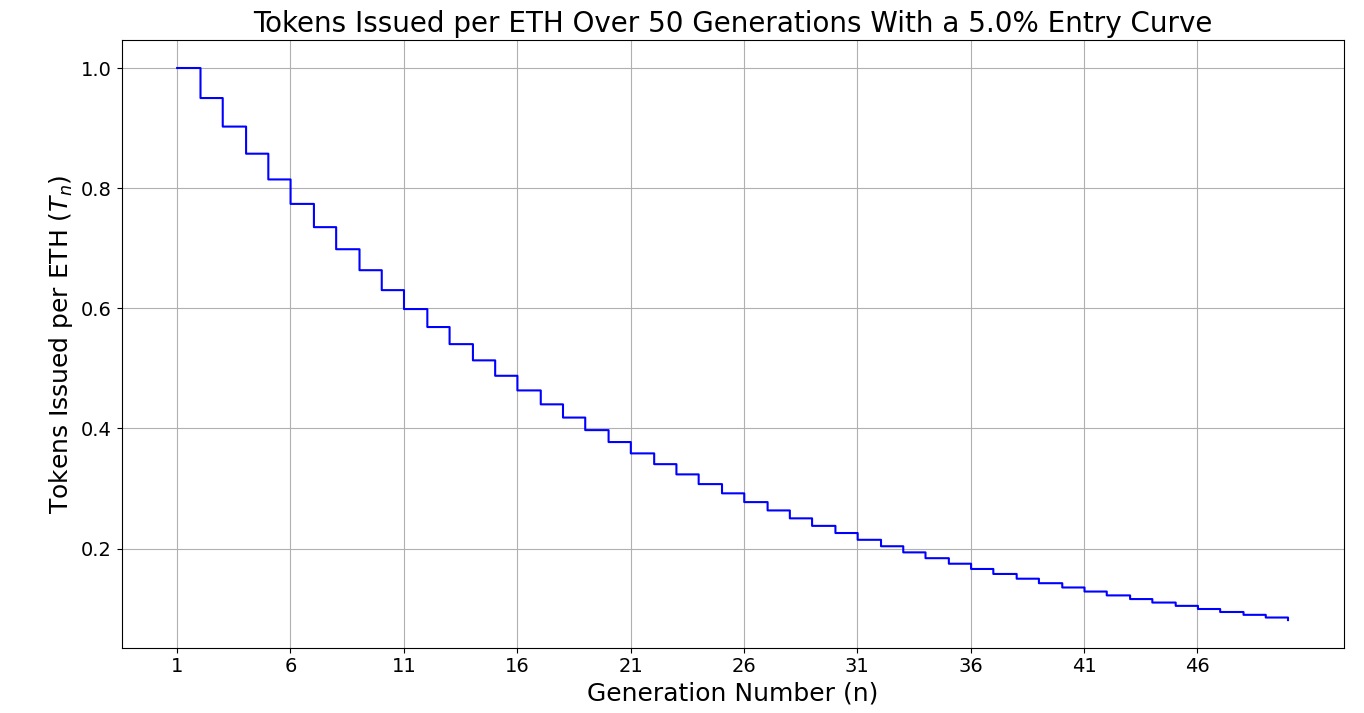
\includegraphics[width=\textwidth]{figures/single-entry-curve.png}
   \caption{This figure shows how $T_n$ (the number of \$tokens issued per ETH in the $n^{th}$ generation) varies across 50 generations with a 5\% price ceiling curve $(r_c = 0.05)$. Note that $T_n$ decreases rapidly at first, then more gradually as $T_n$ tends towards 0 over many generations.}
\end{figure}

\clearpage
\begin{figure}[h]
  \centering
  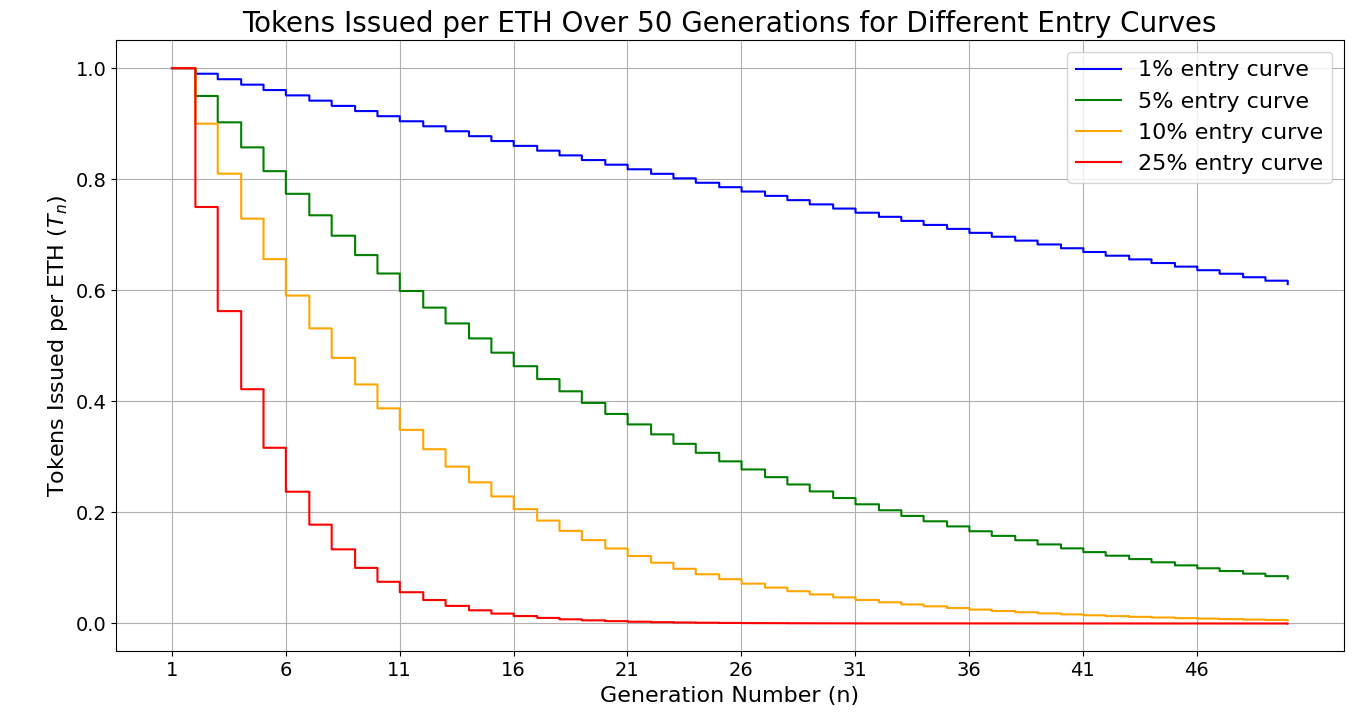
\includegraphics[width=\textwidth]{figures/multi-entry-curves.png}
  \caption{This figure shows how $T_n$ varies over 50 generations with 1\%, 5\%, 10\%, and 25\% price ceiling curves $(r_c = 0.01, 0.05, 0.1, 0.25)$. Note that for greater entry curves, $T_n$ tends towards 0 more quickly.}
\end{figure}

\subsection{Price Floor}

Anyone can destroy their \$tokens to reclaim ETH from the network. The amount of ETH they can reclaim is determined by the price floor function, which is dynamically calculated based on a price floor curve $r_f$ set by the network's creator, the total \$token supply, and the amount of ETH in the network.

The price floor function\footnote{Also see the interactive price floor function on \href{https://www.desmos.com/calculator/9pewqesyj5}{Desmos}} can be expressed as:

\begin{equation}
  V_r = \frac{V_t \times x}{s}\left(\left(1-r_f\right)+\frac{r_f \times x}{s}\right)
\end{equation}

where:
\begin{itemize}
  \item $V_r$ is the amount of ETH which gets reclaimed,
  \item $V_t$ is the total amount of ETH in the network,
  \item $s$ is the total \$token supply,
  \item $r_f$ is the price floor curve (expressed as a decimal), and
  \item $x$ is the number of \$tokens being burned.
\end{itemize}

Unless $r_f$ is 0, this function ensures that as more \$tokens are destroyed (i.e., the larger $x$ is), the more ETH is reclaimed per token.\footnote{If $r_f$ is 0, each \$token will yield the same amount of ETH when destroyed.} This means the first participants to destroy their \$tokens get less ETH per \$token than participants who destroy their \$tokens later. This incentivizes participants to stay in the network longer than other participants in order to increase the amount of ETH they can reclaim.

\begin{figure}[ht]
  \centering
  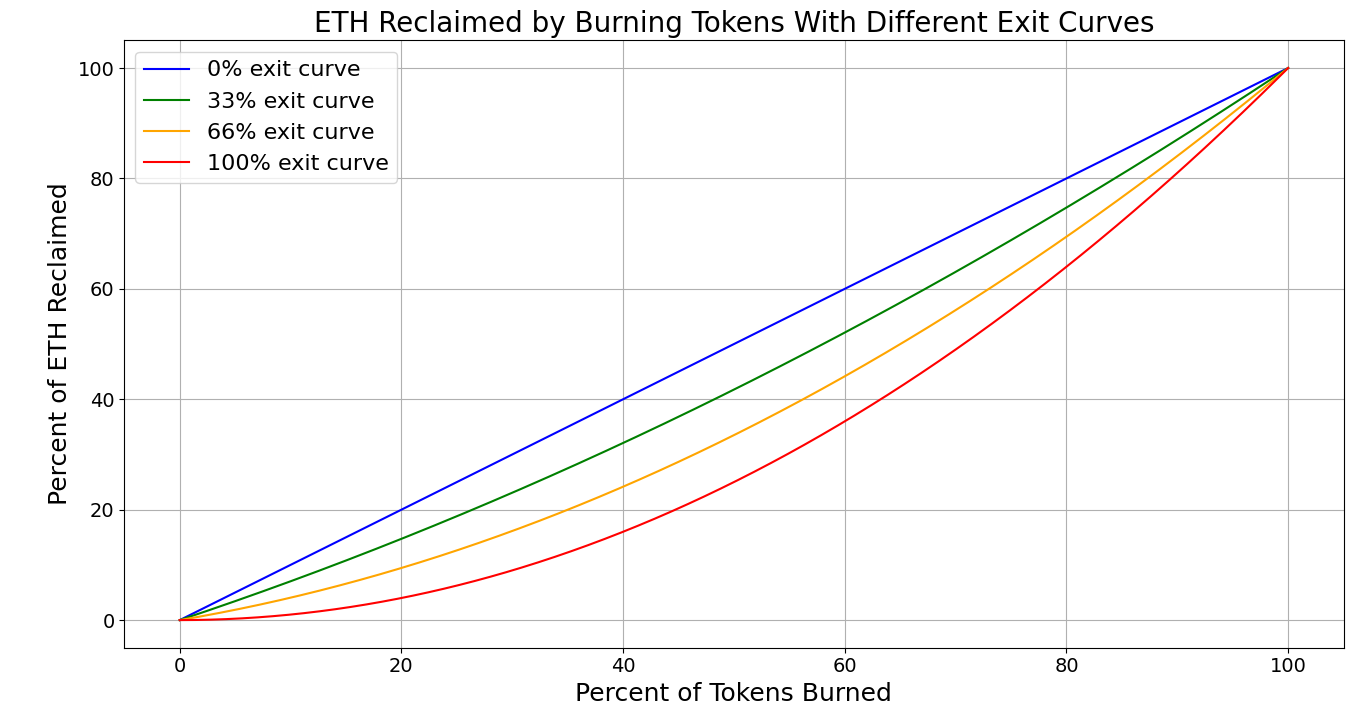
\includegraphics[width=\textwidth]{figures/multi-exit-curves.png}
  \caption{This figure shows price floor functions with price floor curves of 0\%, 33\%, 66\%, and 100\% $(r_f = 0, 0.33, 0.66, 1)$. The $x$ axis represents the percentage of the total \$token supply being destroyed, and the $y$ axis represents the percentage of the network's ETH which is reclaimed. Note that with a 0\% price floor curve $(r_f = 0)$, reclaim amounts are linear with respect to the number of tokens being destroyed---a network participant which destroys \textit{e.g.} 10\% of the total token supply can reclaim 10\% of the network's ETH. The larger the price floor curve, the less ETH earlier reclaimers receive.}
\end{figure}

\section{Contract Implementation}

Revnets are implemented as Solidity smart contracts, and are intended for use on Ethereum, Ethereum L2s,  and other environments with Solidity support. Revnets are built on top of and extend the Juicebox\footnote{See the \href{https://docs.juicebox.money}{Juicebox Docs}.} protocol. Revnets leverage Juicebox's discount rate logic for price ceiling calculations, its redemption logic for price floor calculations, and its reserved rate logic for boost calculations.

While the price of a Revnet's token is between the price ceiling and the price floor, payments are routed to a Uniswap v3 liquidity pool by a Buyback Delegate contract if possible.\footnote{See the Buyback Delegate contracts on \href{https://github.com/jbx-protocol/juice-buyback}{GitHub}.} The Buyback Delegate contract routes incoming payments to the Uniswap pool if doing so would yield more tokens than a payment into the network would create.

Each Revnet is a Juicebox project, which is deployed, owned, and administrated by one of the contracts below.

\begin{table}[h]
  \centering
  \begin{tabular}{|l|c|}
    \hline
    Contract Name & Description \\
    \hline
    \texttt{BasicRetailistJBDeployer} & Deploys a basic Revnet. \\
    \hline
    \texttt{PayAllocatorRetailistJBDeployer} & \\
    \hline
    \texttt{Tiered721PayAllocatorRetailistJBDeployer} & \\
    \hline
  \end{tabular}
  \caption{The Revnet deployer contracts.}
\end{table}

\subsection{BasicRetailistJBDeployer}

Anyone can deploy a basic Revnet by calling the \texttt{BasicRetailistJBDeployer} contract's \texttt{deployBasicNetworkFor(...)} function:

\begin{lstlisting}[language=Solidity]
function deployBasicNetworkFor(
  address _operator,
  JBProjectMetadata memory _networkMetadata,
  string memory _name,
  string memory _symbol,
  BasicRetailistJBParams memory _data,
  IJBPaymentTerminal[] memory _terminals,
  BuybackDelegateSetup memory _buybackDelegateSetup
)
  public
  returns (uint256 networkId)
{ ... }
\end{lstlisting}

This function accepts the following parameters:

\begin{itemize}
  \item \texttt{\_operator} An address that will receive the boost and any pre-minted token. This address has permission to change the boost recipient(s).
  \item \texttt{\_networkMetadata} The Revnet's metadata content and domain (for use in clients).
  \item \texttt{\_name} The name of the ERC-20 token being created for the Revnet.
  \item \texttt{\_symbol} The symbol of the ERC-20 token being created for the Revnet.
  \item \texttt{\_data} A \texttt{BasicRetailistJBParams} struct which specifies the initial token issuance rate for the first generation, the number of tokens which should be pre-minted to the boost address, the generation length, the entry and exit curves, and the boost percentage and duration.
  \item \texttt{\_terminals} The Juicebox payment terminals that the network uses to accept payments.
  \item \texttt{\_buybackDelegateSetup} Info for setting up the buyback delegate to use when determining the best price for new participants.
\end{itemize}

This function deploys and configures the Revnet, deploys the Revnet's ERC-20, premints tokens as needed, and grants the appropriate permissions to the boost address. It then returns a \texttt{networkId}, the Juicebox project ID of the newly created Revnet.

\section{Applications}

% Software projects (like Wikipedia)
% Social networks (like Twitter)
% DAOs
% Insurance
% Public goods
% Artist fan club
% Political activist groups

\subsection{}

\subsection{Software}

Revnets 

\subsection{Social Networks}

\section{Miscellanea}

\subsection{Network Token}

\subsection{Accounting Types}\label{sec:accounting_types}

If the network uses USD-based accounting, payers will receive 1 token per USD worth of ETH under the network's intial conditions. For instance, if the ETH price is 1,000 USD, paying 1 ETH into the network will yield 1,000 tokens.

\subsection{L2s}

\section{Conclusion}

% \bibliographystyle{plain}
% \bibliography{references}

\end{document}

